\section{Návrh metódy}
Navrhovaná metóda zohľadnuje vlastnosti ktoré nie je možné získať iba zo statického obrazu, budeme ich nazívať dynamické príznaky videa.
Avšak metóda stále zohľadnuje v pozorovanom videu aj aspekty statického obrazu, tieto budeme nazívať statické príznaky videa.
Tieto príznaky sú vypočítavané seprátne a nakoniec ich metóda spája do jednej výslednej mapy pozornosti. Výsledkom je postupnosť máp pozornosti pre každý frame videa (podľa vstupnej konfigurácie), ktorý možno spojiť do videa pozornosti pre ľubovolné vstupné video.

\subsection{Dynamické príznaky videa}
Dynamické príznaky metóda najprv extrahuje pomocou štadardnej metódy Horn-Schunck, (referencia na 2 kapitolu alebo na článok?) ktorá vypočíta optický tok na každých 2 rozdielnych framoch videa čím vzniká sémantický príznak pohybu rôznych objektov po scéne spolu s smerovýmy vektormy pohybu daných vektorov.
Získané smerové vektory okamžite spočítavame aby sme získali celkový obraz optického toku pre danú dvojicu obrazov.
Obraz sa následne prahuje statickou konštantou kôli ostráneniu šumu.
Prahovanie prebieha dynamicky vzľadom na počet nájdených 8-spojitých regiónov tj. výstup optikého toku. V našej implementácií je obmedzený počet regiónov na maximálnu hodnotu 200 regiónov.
Prahovanie začne s konštantou ktorú určí pomocou algoritmu Otsu\cite{otsu}, následne určí počet 8-spojitých regiónov akje počet vädší ako maximálna hodnota, zvýši konštantu o 10% z pôvodnej hodnoty.
Tento proces sa opakuje pokial sa v obraze vyskytuje viacej ako maximálny počet regiónov.
Takéto prahovanie je nutné pre optimalizáciu výkonu algoritmu, pretože v prípadoch ked obraz obsahuje veľké množtvo regónov výpočtová rýchlosť algortmu je maximálne neúčinná.
Pixeli s valídnou honotou sa rozdelia na regióny podľa spojitosti a podobnosti štandardným spôsobom.
Pripomenme, že v tomto obraze sa spočítali hodnoty posunu v oboch smeroch aritmeticky do jednej hodnotiacej konštanty (pre každý pixel obrazu), ktorá už nereprezentuje smer posunu daného obrazového pixelu, ale iba hodnotí celkový posun pixelu.
Takto získané regóny budeme vyhodnocovať a spájať podľa pôvodných výsledkov metódy Horn-Schunck.
Vďaka využitiu pôvodných vektorov z výsledku metódy Horn-Schunck, vieme rozlíšiť pohyb horizontálny aj vertikálny separátne.
Pre všetky dvojice regiónov v obraze zistujeme nasledovné charakteristiky:
\begin{enumerate}
  \item\textbf{Rozdiel smerových vektorov v horizontálnom smere}
  \item\textbf{Rozdiel smerových vektorov v vertikálnom smere}
  \item\textbf{Rozdiel vo vzdialenosti}
\end{enumerate}
\subsubsection{Rozdiel smerových vektorov v horizontálnom smere}
Charakteristika sa vypočítava zo smerových horizontálnych vektorov metódy Horn-Schunck.
Pre každý región sa vypočíta maximálna hodnota z indexov daného regiónu.
Následne sa za hodnotu chrakteristiky sa považuje absolútna hodnota rozdielu týchto hodnôt pre každý región.
\begin{equation}
  H_A = max(HS(i_A))
\end{equation}
\begin{equation}
  H_B = max(HS(i_B))
\end{equation}
\begin{equation}
  R_{H} = abs(H_A-H_B)
\end{equation}
Kde A, B reprezentuju všetky dvojice regiónov ktoré sa nachádzajú v obraze.
\begin{math}V_a, V_b\end{math} je maximálna hodnota horizontálnych smerových vektorov z výsledku Horn-Schunck algoritmu pre všetky oblasti patriace danému regiónu.
\begin{math}R_{H}\end{math} je výsledná hodnota charakteristiky.

\subsubsection{Rozdiel smerových vektorov v vertikálnom smere}
Charakteristika sa vypočítava zo smerových vertikálnych vektorov metódy Horn-Schunck.
Prekazdý región sa vypočíta maximálna hodnota z indexov daného regiónu.
Následne sa za hodnotu chrakteristiky sa považuje absolútna hodnota rozdielu týchto hodnôt.

\begin{equation}
  H_A = max(HS(i_A))
\end{equation}
\begin{equation}
  H_B = max(HS(i_B))
\end{equation}
\begin{equation}
  R_{V} = abs(H_A-H_B)
\end{equation}
Kde A, B reprezentuju všetky dvojice regiónov ktoré sa nachádzajú v obraze.
\begin{math}V_a, V_b\end{math} je maximálna hodnota verikálnych smerových vektorov z výsledku Horn-Schunck algoritmu pre všetky oblasti patriace danému regiónu.
\begin{math}R_{V}\end{math} je výsledná hodnota charakteristiky.

\subsubsection{Rozdiel vo vzdialenosti}
Chrakteristika sa vypočítava ako minimálna hodnota vzdialenosti medzi dvojicou regiónov.
Hodnota je počítaná euklidovskou metódou.

\begin{figure}[H]
  \begin{algorithm}[H]
   \ForAll{rohA ako každý extrém regiónu A}{
     \ForAll{rohB ako každý extrém regiónu b}{
      vzdialenost = sqrt( (corner2(1,1)-rohB(1,1))^2 + (rohB(1,2)-rohA(1,2))^2 ) \\
     }
   }
   \caption{Výpočet minimálnej vzdialenosti euklidovskou metódou}
  \end{algorithm}
  \vspace{10mm}
\end{figure}

\subsubsection{Spájanie regiónov}
Po výpočte všetkých 3 charakteristík spojíme všetky dovjice regionov, pre ktoré su všetky chrakteristyky nižšie ako zadefinovaná konštanta.
Regióny spájame pomocou konvexného obalu zjednotenia bodov ležiacich v oboch regiónoch.
\begin{figure}[H]
  \centering
  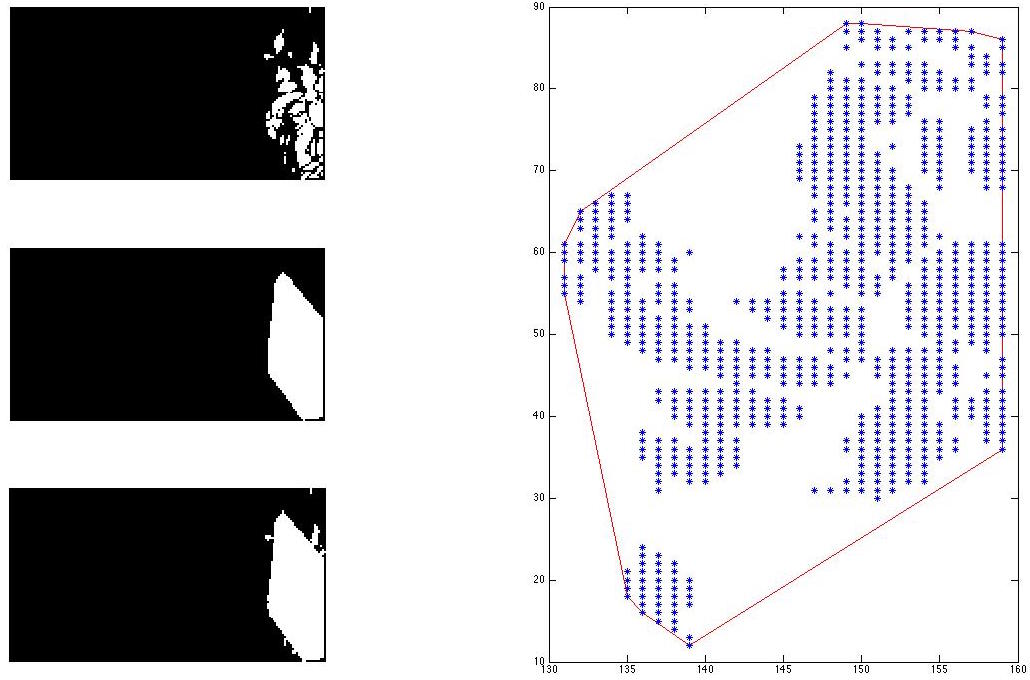
\includegraphics[width=15cm]{pics/spojenie-regionov.jpg}
  \caption{Vyzualizácia spojenia regiónov pomocou konvexného obalu}
  \vspace{10mm}
\end{figure}

\subsubsection{Starnutie objektov na scéne}
Do vypočitavnia dynamických príznakov započítavame predpoklad, že aj pohybujúce sa objekty postupne strácajú pozornosť používateľov.
A to v prípade kedy sa síce daný objekt na scéne pohybuje, ale na identickom mieste.
do metóty zabudujeme mechanizmus kde pixelom s dlhodobo vysokým hodnotením pozornosti, zmenšíme toto hodnotenie pomocou  vynásobenia koeficientom hodnoty \numrange{0}{1}.

\subsection{Statické príznaky videa}
Pri videách kde sa pohybuje celá scéna (kamera je v pohybe) nedávajú dynamické príznaky dobré výsledky kdeže logicky označia celú scénu alebo jej vädšinovú časť scény za výrazne salientnú.
Preto je vhodné dynamické príznaky vhodne kombinovať s klasickýmy modelmy pozornosti ktoré síce zanedbajú postupnosť obrazov, ale nezlyhajú ako dynamické príznaky.
Pre extrakciu statických obrázkov sme zvolili metódu založnú na spektralnych reziduach\cite{spectral-rezidual}.
Vďaka svojmu príncípu potlačovania štatisticky opakujúcich sa predmetov na scéne, sa dá predpokladaď vhodné doplnenie statických objektov ktoré možu zaujať pozornosť na videu ak zlyhávajú dynamické príznaky.

\subsection{Výsledné spojenie príznakov}
Spájanie dynamických a statických príznakov bude prebiehat pomocou sčítania oboch máp, pričom vždy s použijú v určitom pomere.
Výpočet pomeru bude určovať pomer výskytu salientných pixelov v mape dynamických príznakov.

@TODO add latex som symbol \\
\begin{equation}
  pomer = (sum(P_D} > 0))/Pix_{count}
\end{equation}
Kde \begin{math}P_D\end{math} reprezentuje mapu dynamických príznakov a \begin{math}Pix_{count}\end{math} je počet všetkých pixelov ktoré obraz obsahuje.

Ak je vysoký výskyt salientých pixelov, potrebujeme utlmit zobrazovanie tejto časti príznakov a prioritizovať zobrazovanie statických priznakov preto zmiešavacia funkcia vyzerá nasledovne:

\begin{equation}
  Výsledok = (P_D * (1-pomer)) + (P_S * pomer)
\end{equation}
Kde \begin{math}P_D\end{math} reprezentuje mapu dynamických príznakov a \begin{math}P_S\end{math} mapu statických príznakov.

V prípade, že algoritmus nedokáže detekovať žiadny pohyb na scéne, bol by model pozornosti prázdny.
Preto v prípade keď je vyššie spomýnaný pomer dynamických pixelov extrémne nízky použijeme ako výstup algoritmu iba statické príznaky.
Naopak v prípade, že kamera je v pohybe Horn-Schunck algoritmus označí ako pohybujúci sa vädšinovú oblasť obrazu a v tom prípade je potrebné utlmiť dynamické príznaky obrazu a do popredia vystupujú statické.

\subsection{Zdrojové kodý modelu}
Zdrojový kód obsahuje jednu metódu ktorá príma na vstupe vždy 2 parametre.
Prvý parameter je aktuálny frame videa a druhý parameter je frame videa určený na extrakciu dynamických príznakov videa pomocou differencie vzľadom na prvý obrazový frame.
Tieto 2 obrazové vstupy nemusia byť nutne po sebe idúce, je na používateľovy či použije model serializovane na každý frame videa, alebo zvolí vlastnú implementáciu keyframingu (napríklad kôli časovej náročnosti algoritmu).
Algoritmus je schopný processovať farebné aj čiernobiele obrazové vstupy.
V prílohe je možné nájsť 2 implementácie a to implementáciu ako modelu pre applikáciu na porovnávanie modelov načítavajúca kažké 2 posebeidúce obrazové framy.
Druhá implementácia načítava na vstupe priamo video a na výstup dá video s korešpondujúcim videom význačných oblastí, tátoimplementácia je určená na použitie mimo aplikácie na testovanie.
Obe implementácie sú dostupné v prílohe na CD alebo voľne dostupné na internete.

\clearpage

\subsection{Pipeline metódy}
  Grafický popis metódy obsahujúci príklad zostavenia mapy pozornosti.

  \begin{figure}[H]
    \centering
    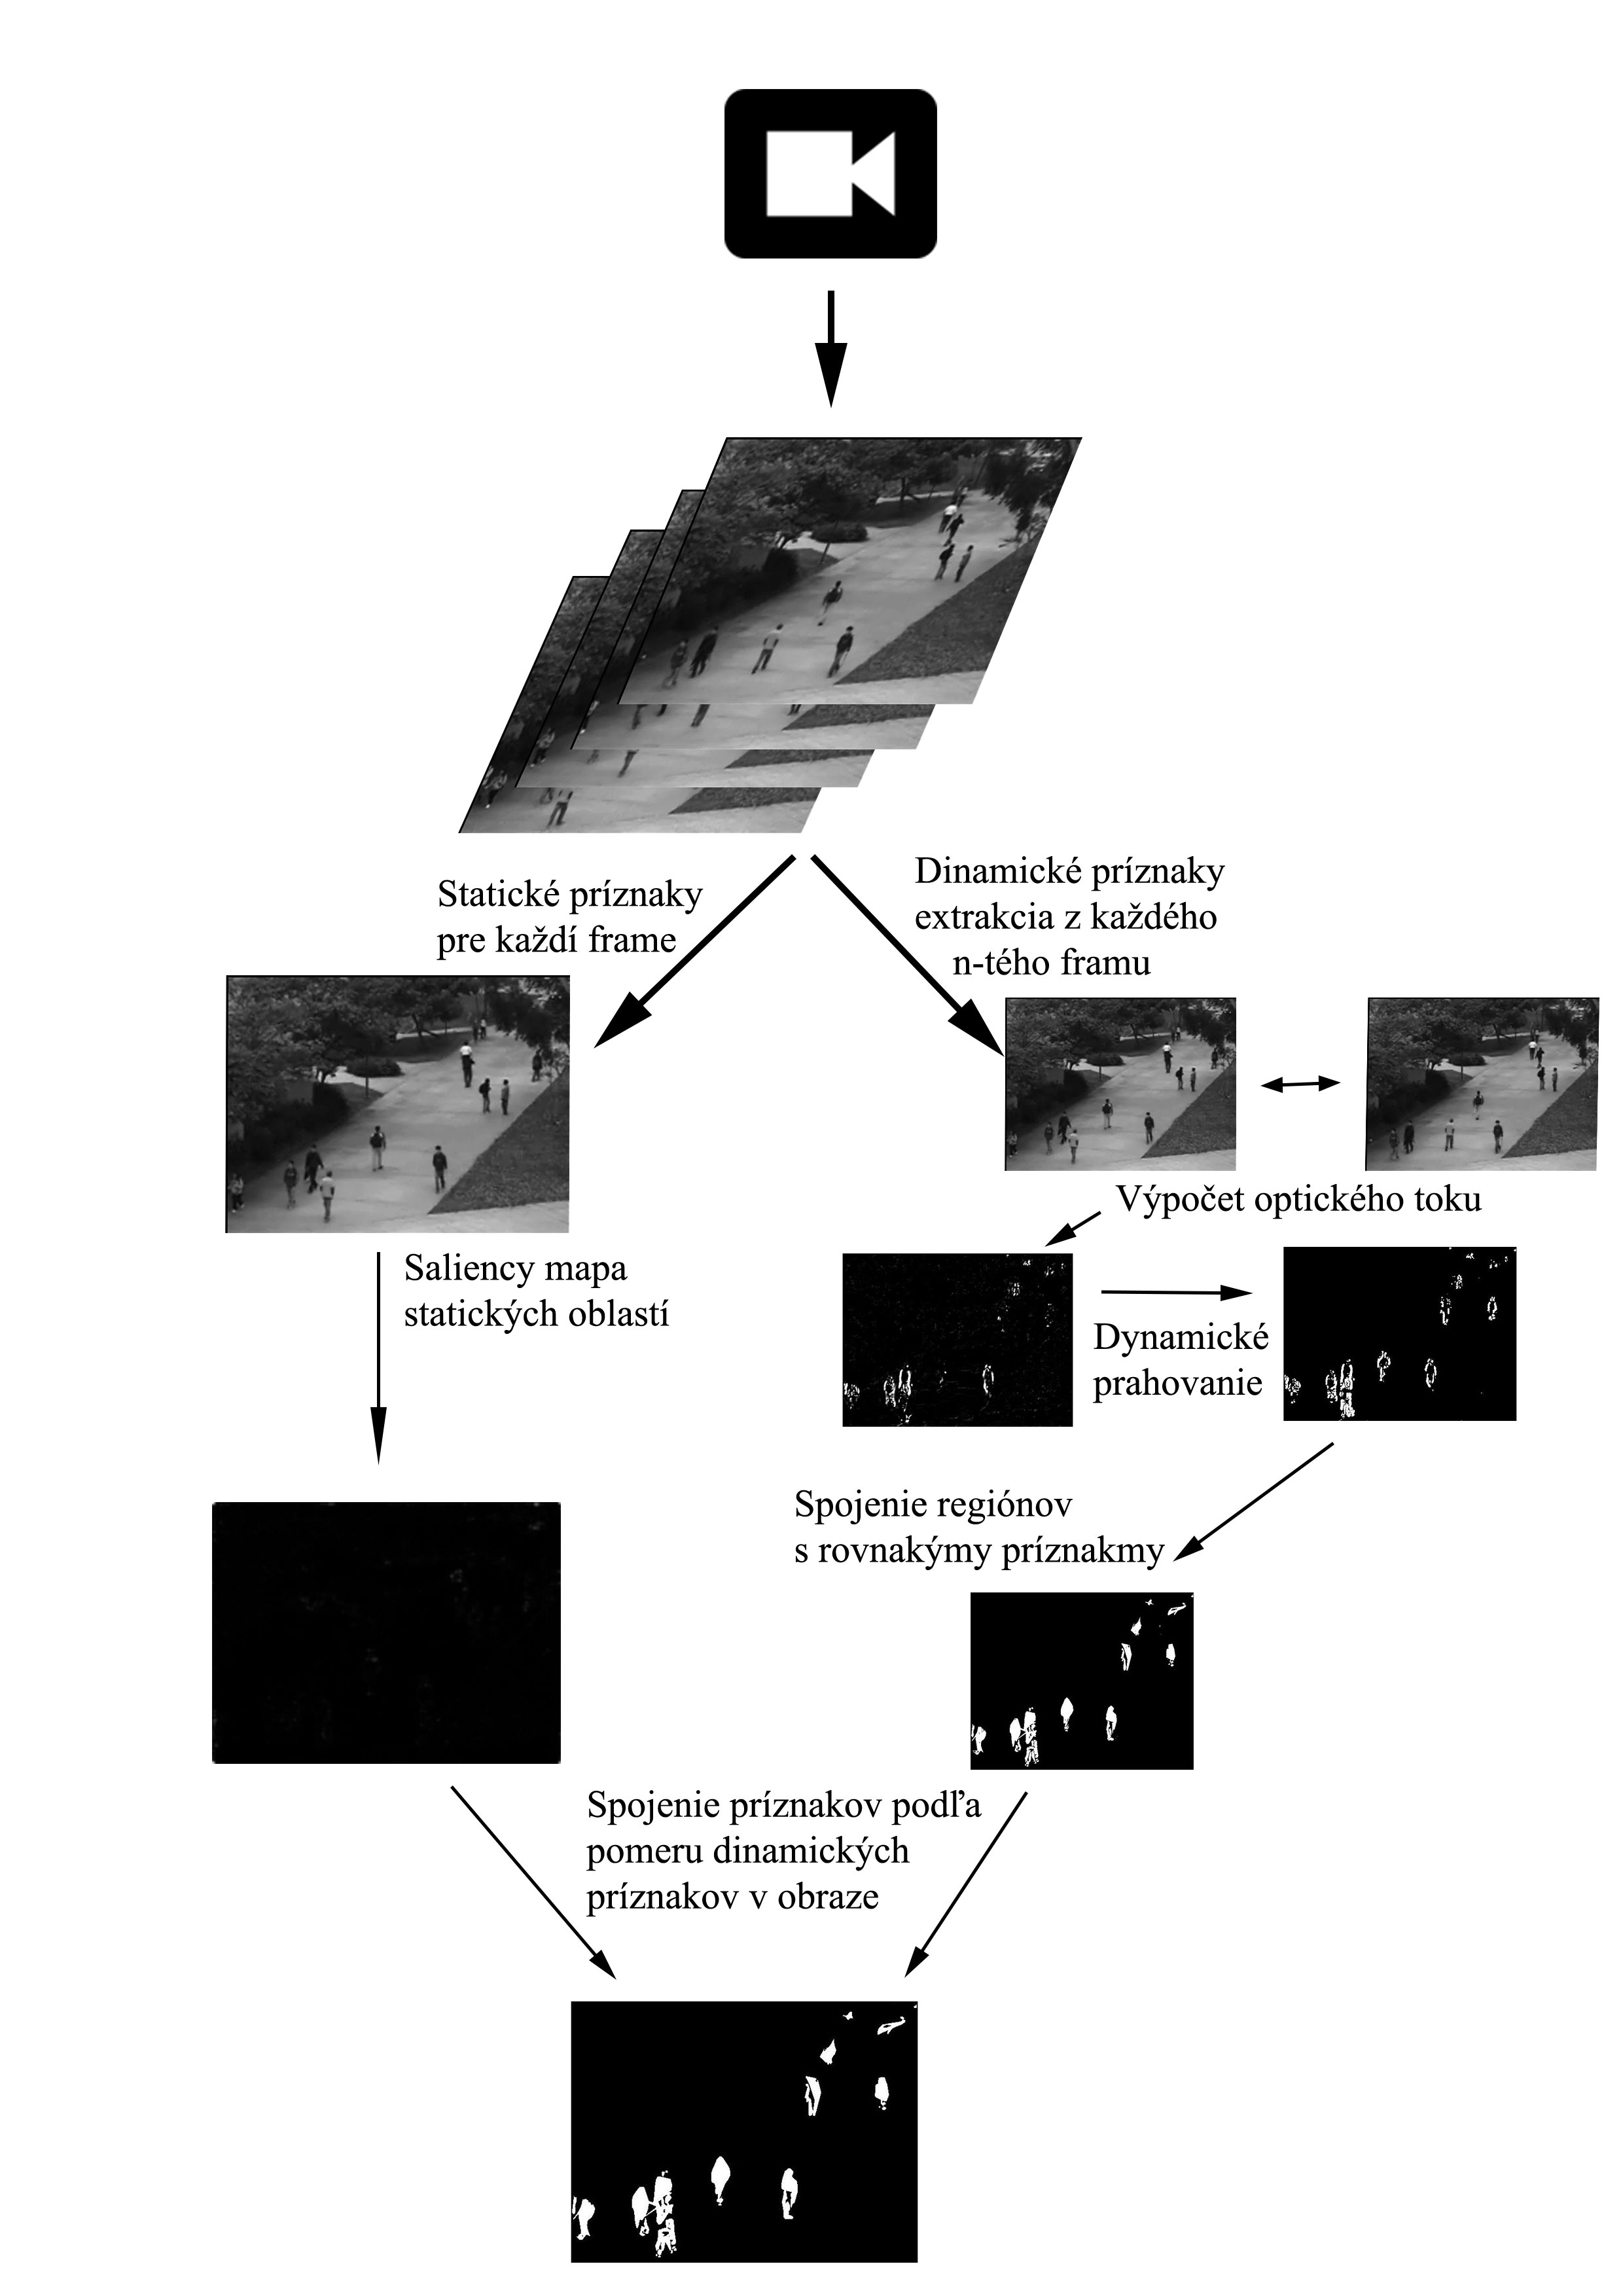
\includegraphics[width=15cm]{pics/workflow.jpg}
    \caption{Ucelená vyzualizácia algoritmu}
    \vspace{10mm}
  \end{figure}

\section{Implementácia riešenia}
Implementácia vyššie uvedeného algoritmu je implementovaná ako modul pre aplikáciu na porovnávanie a  automatickú validáciu výsledkov.
Aplikácia na porovnávanie je takisto implementovaná v prostredí matlab.

\subsection{Aplikáciu na porovnávanie a automatickú validáciu}
Sekundárnym prínosom práce je vytvorenie aplikácie pre zjednodušenie budúcej práce pri prototypovaní nových modelov pozornosti.
A následné uľahčenie validačného procesu pre potencionálnych vývojárov.\\
Základná functionalita:
\begin{enumerate}
  \item\textbf{Oddelenie logiky testovnia a logiky samotného modelu}
  \item\textbf{Simultálne sledovanie videa z viacerých modelov}
  \item\textbf{Automatická validácia modelu}
  \item\textbf{Vizualizácia výsledkov validácie}
\end{enumerate}

\subsubsection{Oddelenie logiky testovnia a logiky samotného modelu}
V aplikácií na testovanie je možné pripdávať lubovolné modeli pre ktoré je dostupná implmentácia v jazyku matlab.
Pre iné jazyky je potrebné doprogramovat wrapper ktorý spustí daný jazyk a vypočíta mapu pozornosti.
Ukážkový wrapper je súčastou aplikácie.
Pre pripadnie nového modelu je potrebné pridať wrapper do zložky "models", knižnice vyžadované modelmi je potrebné skopírovat do lubovolnej podzložky tohoto priečinka.
Pri spustení apikácie sa načítaju všetky moduli aj kničnice uložené v podzložkách.

\subsubsection{Simultálne sledovanie videa z viacerých modelov}
Pre rýchle prototypovanie je vhodné pozorovať rovnaké video pri rôznych úpravách.
Táto funkcionalita je dostupná pre každý model s vygenerovanýmy mapamy pozornosti na zvolenom videu.

\subsubsection{Automatická validácia modelu}
Validovanie výsledokov je nutnou súčastou každého modelu pozornosti preto aplikácia ponúka automatizovaný spôsob ako zvalidovať výsledky na vybraných referenčných datasetoch.
Validácia tvorí pre kažké video perzistentný súbor obsahujúci 3 metriky: AUC-Judd, KL-Div, NSS.
Vyššie spomenuté metriky sa rátajú pre každý frame videa.
Validácia prebieha paralelne pre všetky videá zvoleného datasetu.
Vytvorené súbory sú perzistetné z dôvodu dlhého výpočtového času, a ukladajú sa do priečinku results a podložky podľa názvu testovaného datasetu v tvare \begin{math}názovModelu.názovDatasetuČísloVidea.mat\end{math}.
Formát súboru obsahuje 3 premenné s názvamy: AUROC\_score, KLDIV\_score, NSS\_score.
Každá premenná obsahuje pole podla dĺžky videa (počet frameov) a hodnotami danej metriky.
Aplikácia aktuálne podporuje 2 datasety a to: ASCMN\cite{accv}, coutrotove testovacie datasety #1\cite{coutrot-database} a #2\cite{coutrot-database-2}, tieto datasety sú volne dostupné a súčastou aplikácie je programový kód slúžiaci na načítanie a validovanie výsledkov (samotné vstupné videá a fixácie je potrebné stiahnuť zo stránky autorov)
Dataset ASCMN\cite{accv} je poskytovaný autormy aj s testovacím algoritmom na výpočet vyššie uvedených metrík, do aplikácie na testovanie bol iba pozmenený pre načítanie ľubovolného modelu a prisposobený na paralelný vypočet všetkých videí paralelne.
Pre Coutrot datasety aplikácia na tstovanie obsahuje upravenú verziu validačného algoritmu z datasetu ASCMN.

\subsubsection{Vizualizácia výsledkov validácie}
Pre analýzu výsledkov validácie dokáže aplikácia prehladne vyzualizovať všetky dáta získané testovaním.
Vyzualizácie sú súčastou validácie v daľších kapitolách.

\subsection{Implementácia modulu}
Implementácia nového modelu pozornosti je jednoduchá.
Pre integrovanie ľubovolného modelu je možné použiť vzorovú implementáciu ktorá je dostupná v prílohách.

\section{Validácia výsledkov}
Validácia vyššie spomínaného modelu prebiahala pomocou automatického testovania v aplikácií na testovanie.
Prezentovať budem výsledky z nasledujúch datasetov: \textbf{ASCMN\cite{accv}}, \textbf{Coutrot #1\cite{coutrot-database}}, \textbf{Coutrot #2\cite{coutrot-database-2}}.
Výsledky budem hodnotiť pomocou nasledkujúcich metrík: \textbf{AUCROC\cite{metrics-1}}, \textbf{KLDIV\cite{metrics-1}}, \textbf{NSS\cite{metrics-1}}.
V nasledujúcich sekciách budem prezentovať výsledky validácie pre navrhovaný model a dalej vyhodnocovať vytvorený benchmark.
\\
\\
@TODO screens+postup of validation???
\\
\\
\subsection{Analýza výsledkov}
V tejto sekcií budem prezentovať výsledky všetkých datasetov vzhľadom na navrhovaný model.
Výsledky budem vyzualizovať pomocou chrakteristiky vzniknutej zo strednej hodnoty framov, jednotlivých videí.
Kažká metrika bude vyhodnocovaná samostane. Ako prvý budeme analyzovať dataset ASCMN\cite{accv} a následne oba Coutrotove datasety.

\subsubsection{ASCMN}
\begin{figure}[H]
  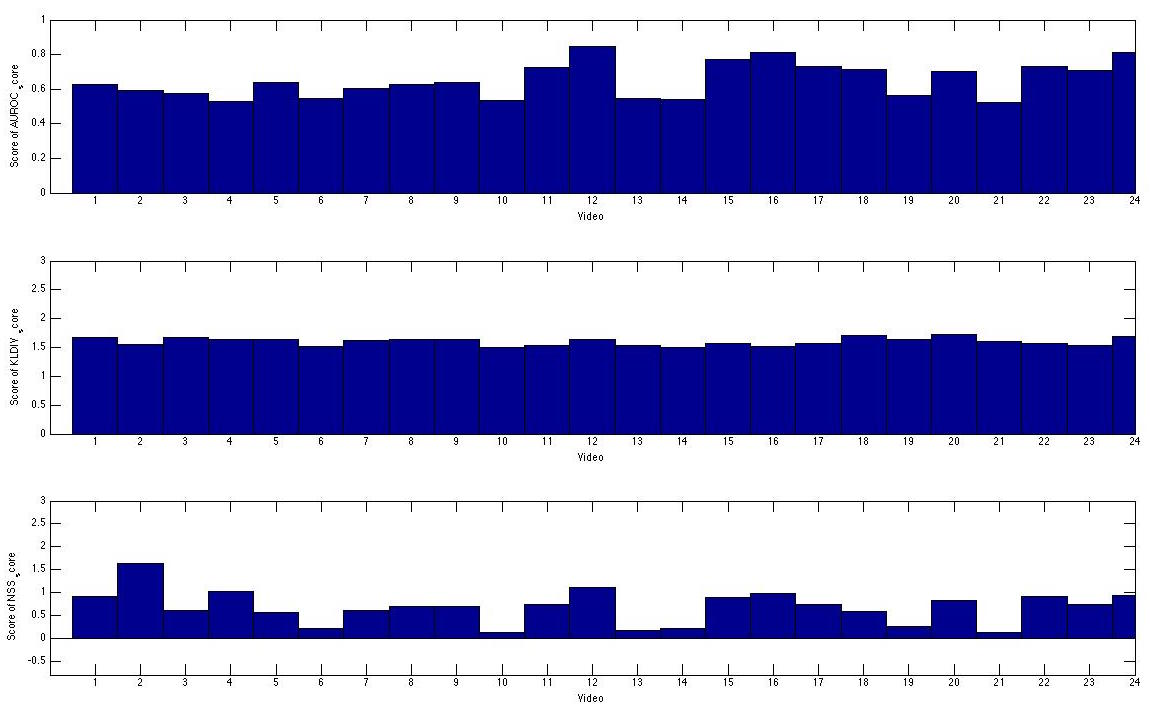
\includegraphics[width=15cm]{pics/single-accv.jpg}
  \caption{Vyzualizácia všetkých testovaných metrík pre dataset ASCMN\cite{accv} pre jednotlivé videá}
  \label{fig:ASCMN1}
\end{figure}

\subsubsection{ASCMN - AUCROC}
Ideálna hodnota tejto metriky je 1, čo reálne značí 100\% úspešnosť.
Náhodná mapa pozornosti má hodnotu 0.5, z toho dôvodu aby sme dokázali správnosť nového modelu potrebujeme dokázať, že model má hodnotu AUC v intervale \interval[{0.5,1}].
Z grafu \ref{fig:ASCMN1} vyplýva, že všetky videá spĺnaju vyššie uvedenú podmienku.
Graf \ref{fig:ASCMN2} už priamo dokazuje túto hypotézu keďže ho tvorí stredná hodnota všekých testovaných videí.
Výsledná hodnota AUC 0.651, je hodnota dostatočne vyššia ako 0.5.
takáto hodnota vyhodnocuje náš model ako korelujúci s reálne nameranýmy dátamy na používateľoch zúčastnených sa na tvorbe tohoto datasetu.
\subsubsection{ASCMN - KLDIV}
Ideálna hodnota tejto metriky je 0, čo reálne značí že saliency mapa je totožná s ground truth mapou.
Výsledné hodnoty pre všetky videá sa podľa grafu \ref{fig:ASCMN1} pohybujú v intervale \interval[{1.5,1.7}].
Hodnoty menšie ako 2 značia tiež koreláciu s reálnymy dátamy.
Výsledná hodnota KLDIV je 1.602 je nižsia ako 2, preto aj metrika KLDIV úspešne validuje náš model vrámci datasetu.
\subsubsection{ASCMN - NSS}
Výsledná hodnota NSS je 0.680.

\subsubsection{Coutrot #1}
\begin{figure}[H]
  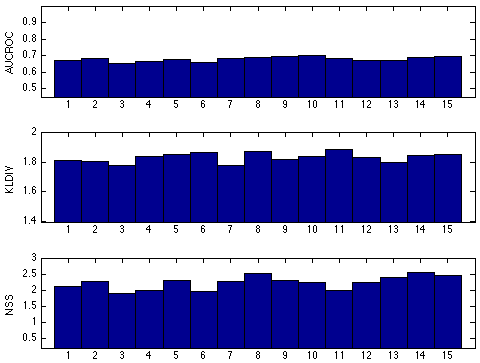
\includegraphics[width=15cm]{pics/single-coutrot1.png}
  \caption{Vyzualizácia všetkých testovaných metrík pre dataset ASCMN\cite{accv} pre jednotlivé videá}
  \label{fig:coutrot1}
\end{figure}
\subsubsection{Coutrot #1 - AUCROC}
\subsubsection{Coutrot #1 - KLDIV}
\subsubsection{Coutrot #1 - NSS}

\subsubsection{Coutrot #2}
\begin{figure}[H]
  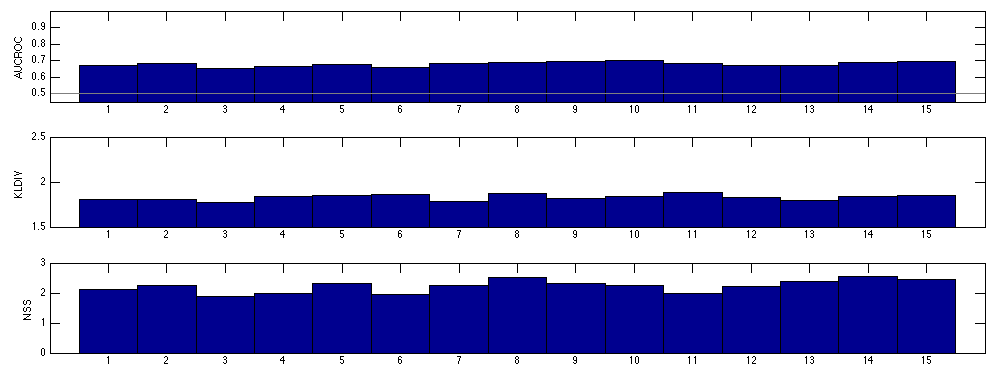
\includegraphics[width=15cm]{pics/single-coutrot2.png}
  \caption{Vyzualizácia všetkých testovaných metrík pre dataset ASCMN\cite{accv} pre jednotlivé videá}
  \label{fig:coutrot1}
\end{figure}
\subsubsection{Coutrot #2 - AUCROC}
\subsubsection{Coutrot #2 - KLDIV}
\subsubsection{Coutrot #2 - NSS}

\subsection{Porovnávanie s konkurenčnýmy modelmy pozornosti}
Porovnanie s konkurenciou nám poskytne dalšie relevantné poznatky.
Budeme sa konkrétne snažiť dokázať ze efektivita našeho nového modelu je vyššia ako povodného horn-struck algoritmu\cite{horn-schunck}, používaného na extrakciu dynamickej zložky príznakov.
Zároveň sa budem snažiť o dôkaz, že algoritmus je efektívnejší aj ako samotná statická zložka ktorá je vypočítavaná pomocou modelu Spektralnych rezidual\cite{spectral-rezidual}.
Pre tento účel som uskutočnil benchmark obsahujúci nasledovné algoritmy:
\begin{enumerate}
  \item\textbf{AttentionSimpleGlobalRarity\cite{global-rarity}}
  \item\textbf{AttentionSimpleLocalContrast\cite{global-rarity}}
  \item\textbf{FES\cite{fes}}
  \item\textbf{RARE\cite{rare-1}}
  \item\textbf{Horn-struck\cite{horn-schunck}}
  \item\textbf{Lucas-Kanade\cite{lucas-kanade}}
  \item\textbf{Spektralne rezidua\cite{spectral-rezidual}}
\end{enumerate}
na všetkých datasetoch.
Ku každému datasetu uvedieme 2 súhrnné štatistiky.
Prvá vyjadruje porovnanie priemernej hodnoty každej z metrík pre kažkdé video samostatne, druhá obsahuje priemerné hodnoty všetkých videií, pre všetky testované medódy.

\begin{figure}[H]
  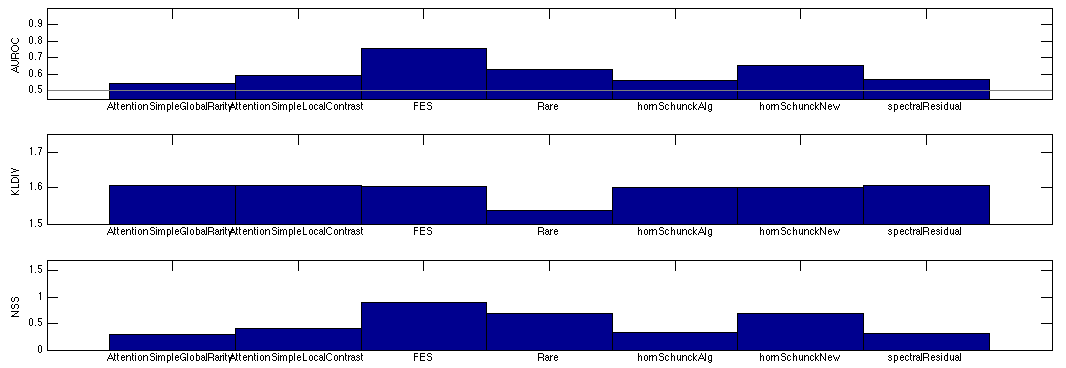
\includegraphics[width=15cm]{pics/porovnanie-accv-global-new.png}
  \caption{Vyzualizácia porovnania pre dataset ASCMN\cite{accv}}
\end{figure}

\subsubsection{ASCMN}
\begin{figure}[H]
  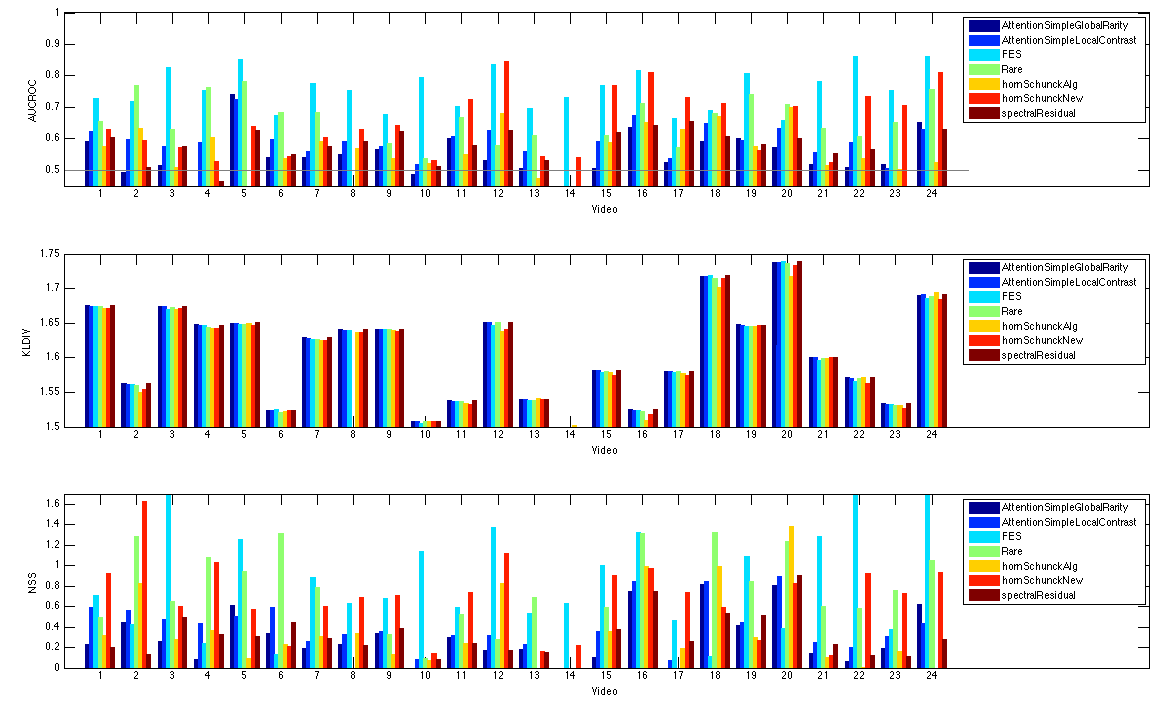
\includegraphics[angle=90, width=14cm]{pics/porovnanie-accv-new.png}
  \caption{Vyzualizácia porovnania pre dataset ASCMN\cite{accv}}
\end{figure}

\subsubsection{Coutrot #1}
\begin{figure}[H]
  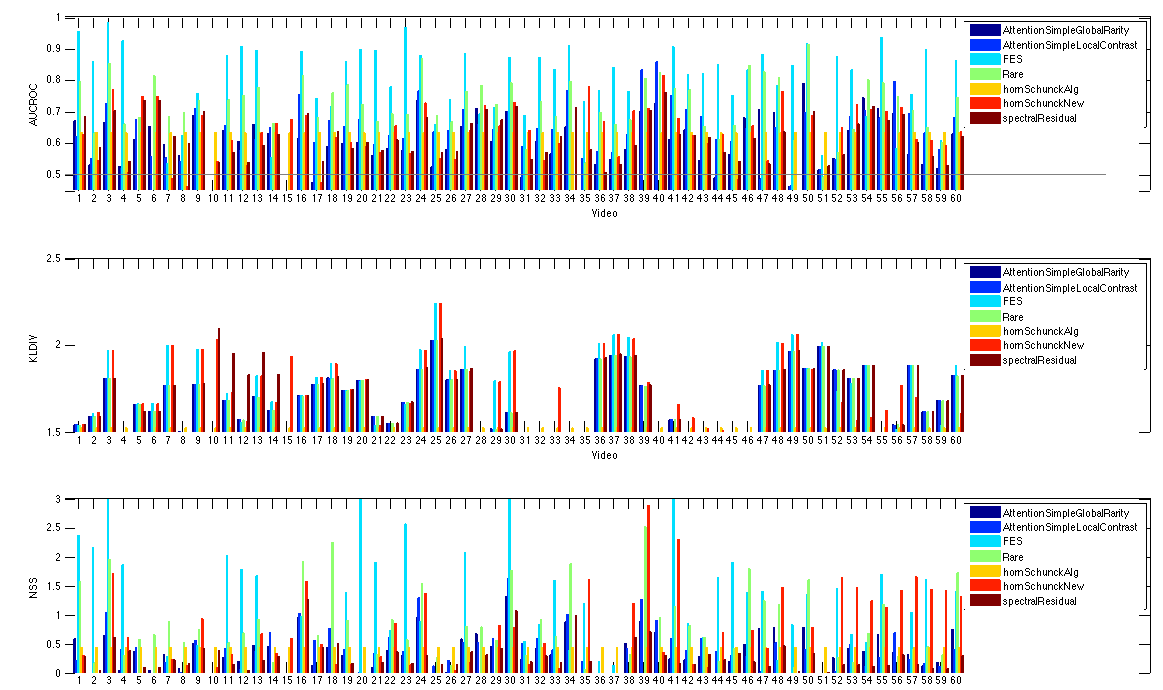
\includegraphics[angle=90, width=15cm]{pics/porovnanie-coutrot1.png}
  \caption{Vyzualizácia porovnania pre dataset ASCMN\cite{accv}}
\end{figure}

\begin{figure}[H]
  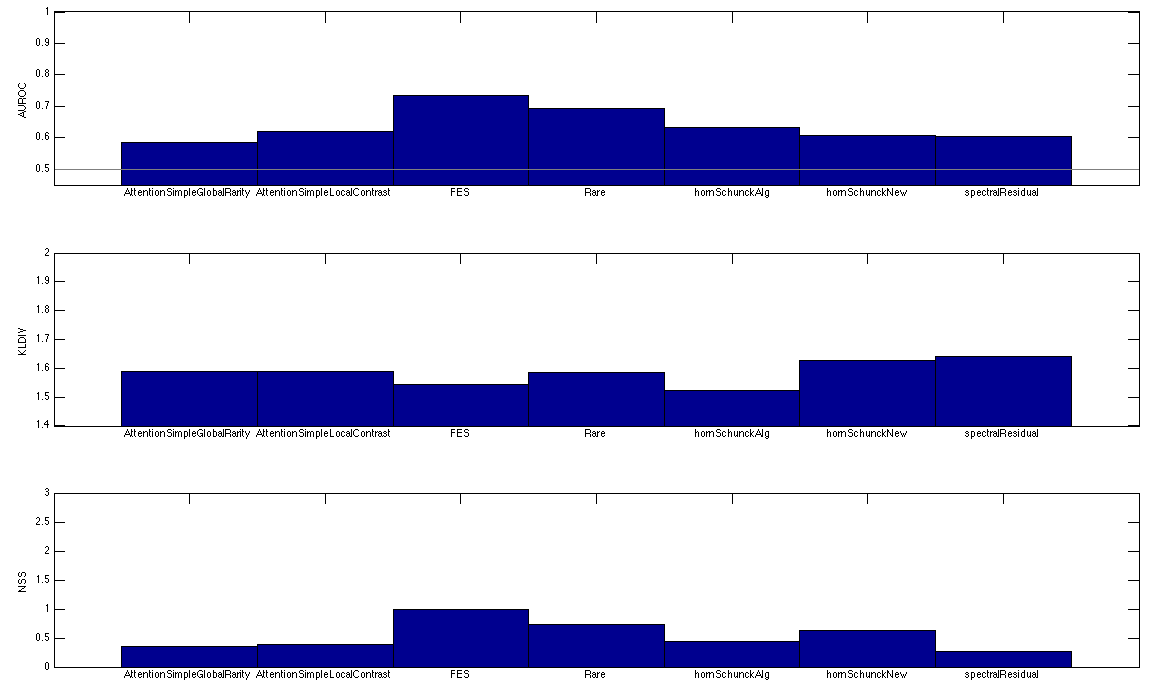
\includegraphics[width=15cm]{pics/porovnanie-coutrot1-global.png}
  \caption{Vyzualizácia porovnania pre dataset ASCMN\cite{accv}}
\end{figure}


\subsubsection{Coutrot #2}
\begin{figure}[H]
  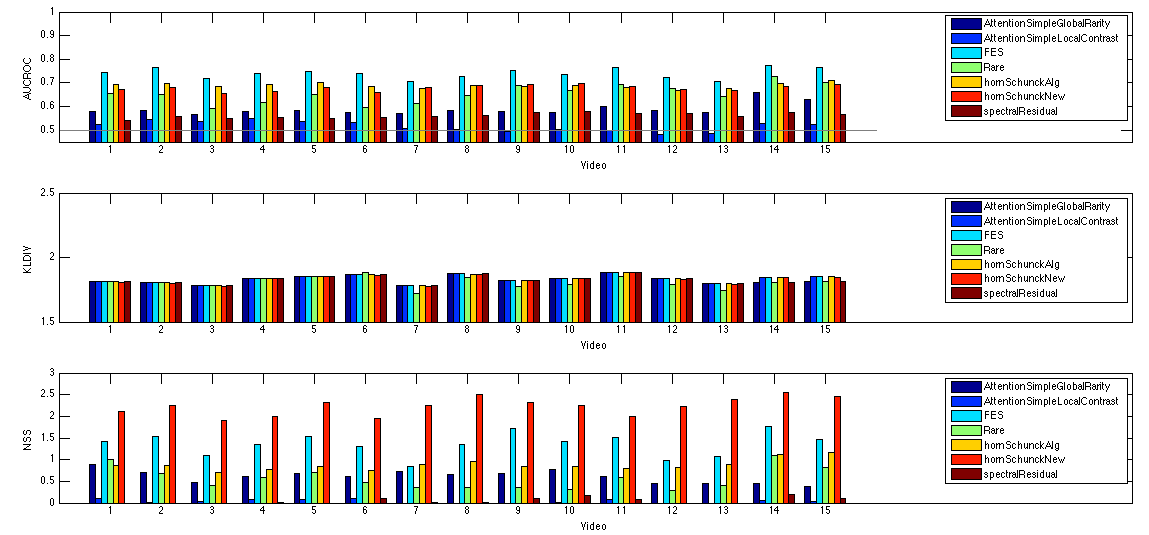
\includegraphics[angle=90, width=15cm]{pics/porovnanie-coutrot2.png}
  \caption{Vyzualizácia porovnania pre dataset ASCMN\cite{accv}}
\end{figure}

\begin{figure}[H]
  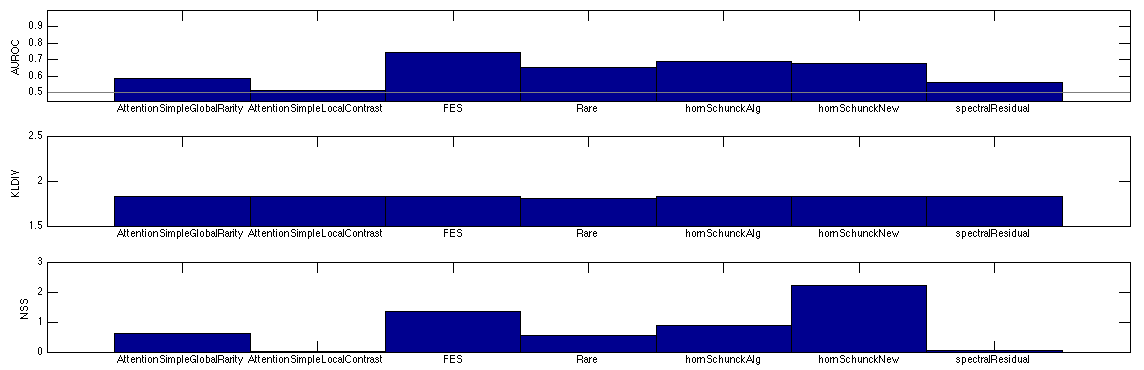
\includegraphics[width=15cm]{pics/porovnanie-coutrot2-global.png}
  \caption{Vyzualizácia porovnania pre dataset ASCMN\cite{accv}}
\end{figure}

\subsection{Zhrnutie validacie}
Všetky metriky potvrdzuju tvrdenie, že narvhovaný model ma značnú koreláciu k skutočným dátam nameraných na reálnych užívateľoch.
Zároveň validácia bola prevedená na typovo rozdielnych videách, keďže videá obsahujú pohybujúcu sa kameru aj statickú pozíciu kamery, konverzačné scény aj scény s prírodnýmy motívamy.
Zároveň na základe vypracovaného benchmarku možeme tvrdiť, že nová metóda je efektívnejšia ako základné metódy použité na získanie dynamických aj statických príznakov.

\section{Diskusia}
Možnosť na zlepšenie algoritmu vidieť, v celom benchmarku kde model Rare\cite{rare-1} dosahoval výrazne lepšie výsledky aj napriek používaniu iba statických príznakov.
Daľšia možnosť ako vylepšiť je v rýchlosti spracovania ktorá nie je použiteľná na realtime spracovanie obrazu.
Algoritmus je svojou časovou náročnostou vhodný na spracovanie videan v nízkej obrazovej kvalite.
Avšak pri vysokej obrazovej kvalite, algoritmus nevykazoval vyššiu efektovitu (otestované na datasete savam\cite{savam} ktorý poskytuje videá vo vysokej kvalite).
Ale výpočet trval výrazne dlhšie ako v porovnaní s videom s nízkou obrazovou kvalitou.
Daľšiu možnosť pre zlepšenie odhaluje validácia datasetu Coutrot #2, kde pôvodný algotritmus horn-struck dosiahol hodnotenie porovnateľné v navrhovaným modelom.
Takéto výsledky sú spôsobené výberom rozostupu frameov (podla ktorých sa počíta dynamická zložka).
Keďže rozpetie bolo zvolené na každú dvojicu framov pri týchto videách sa často stávalo, že algoritmus detekoval iba minimálny pohyb.
Čo bolo považované za šum a z toho dôvodu bola dymamická zložka potlačená alebo úplne eliminovaná (čo bolo v tomto prípade chybné).
Riešením by bolo porovnávanie viacej framov a následná extrakcia pohybu všetkých dvojíc dokopy.
Tento postup by už nebol považovaný za šum a dynamická zložka by nebola elliminovaná.
